% Copyright 2004 by Till Tantau <tantau@users.sourceforge.net>.
%
% In principle, this file can be redistributed and/or modified under
% the terms of the GNU Public License, version 2.
%
% However, this file is supposed to be a template to be modified
% for your own needs. For this reason, if you use this file as a
% template and not specifically distribute it as part of a another
% package/program, I grant the extra permission to freely copy and
% modify this file as you see fit and even to delete this copyright
% notice. 

\documentclass{beamer}

% There are many different themes available for Beamer. A comprehensive
% list with examples is given here:
% http://deic.uab.es/~iblanes/beamer_gallery/index_by_theme.html
% You can uncomment the themes below if you would like to use a different
% one:
%\usetheme{AnnArbor}
%\usetheme{Antibes}
%\usetheme{Bergen}
%\usetheme{Berkeley}
%\usetheme{Berlin}
%\usetheme{Boadilla}
%\usetheme{boxes}
%\usetheme{CambridgeUS}
%\usetheme{Copenhagen}
%\usetheme{Darmstadt}
%\usetheme{default}
%\usetheme{Frankfurt}
%\usetheme{Goettingen}
%\usetheme{Hannover}
%\usetheme{Ilmenau}
%\usetheme{JuanLesPins}
%\usetheme{Luebeck}
\usetheme{Madrid}
%\usetheme{Malmoe}
%\usetheme{Marburg}
%\usetheme{Montpellier}
%\usetheme{PaloAlto}
%\usetheme{Pittsburgh}
%\usetheme{Rochester}
%\usetheme{Singapore}
%\usetheme{Szeged}
%\usetheme{Warsaw}


\title{eBPF 101}

%\pgfdeclareimage[height=2.3cm]{cerc-logo}{cerc.png}
%\pgfdeclareimage[height=0.6cm]{university-logo}{iiitd-logo.png}

% A subtitle is optional and this may be deleted
\subtitle{An overview from a perspective of a non-kernel programmer}

%\author[@vimfrw]{Muhammad Falak R~Wani }%\inst{falakreyaz@gmail.com}}  
%\institute[falakreyaz@gmail.com]{}
\author[@vimfrw]{\texorpdfstring{Muhammad Falak R~Wani\newline\url{falakreyaz@gmail.com}}{Author}}

% \institute[Microsoft] {Microsoft} % (optional, but mostly needed)
%{
%%  Cybersecurity Education and Research Centre -- {\em (CERC)} \\
%  Department of Computer Science\\
%  IIIT-D\\
%%  \centering
%%  \pgfuseimage{cerc-logo}
%
%}

\date[LCA 22]{Linux Conf Au 2022}

\subject{eBPF}

% If you have a file called "university-logo-filename.xxx", where xxx
% is a graphic format that can be processed by latex or pdflatex,
% resp., then you can add a logo as follows:

%\logo{\pgfuseimage{university-logo}}

% Delete this, if you do not want the table of contents to pop up at
% the beginning of each subsection:
%\AtBeginSubsection[]
\AtBeginSection[]
{
	\begin{frame}<beamer>{Agenda}
		%\tableofcontents[currentsection,currentsubsection]
		\tableofcontents[currentsection]
	\end{frame}
}

% Let's get started
\begin{document}

\begin{frame}
	\titlepage
\end{frame}

\begin{frame}{Agenda}
	\tableofcontents
	
	% You might wish to add the option [pausesections]
\end{frame}

% Section and subsections will appear in the presentation overview
% and table of contents.
\section{History}

\subsection{Motivation}

\begin{frame}{whoami}{I admit I am an imposter}
    \centering
    
\includegraphics[height=7cm]{imposter.png}
\end{frame}


\begin{frame}{Let's design a Packet Filter}{How hard can that be?}
\begin{columns}[T]
\begin{column}{0.4\textwidth}
\begin{center}
      \begin{itemize}
      \item \LARGE{Copy everything to user-space}
      \end{itemize}
     \vspace{15mm} 
      \begin{itemize}
      \item \LARGE{Write a Kernel Module}
      \end{itemize}
\end{center}
\end{column}
\begin{column}{0.6\textwidth}
      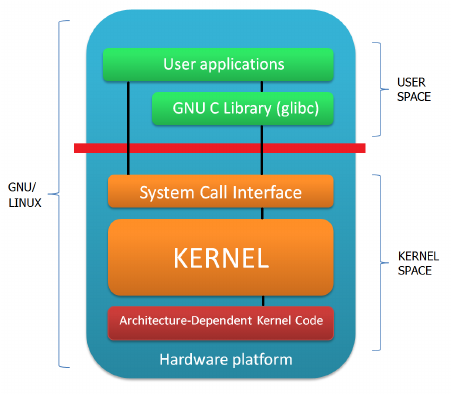
\includegraphics[height=6cm]{userspace-kernelspace.png}
\end{column}
\end{columns}

%\pause
%\vfill{}
%{\Large But wait! \\VM's also do the same...}
\end{frame}

\subsection{Problem}

\begin{frame}{What is the Problem?}{User Space vs Kernel Space Trade Off}
\begin{columns}
\begin{column}{0.5\textwidth}
\begin{center}
User Space
\end{center}
\begin{itemize}
    \item We copy every packet to User Space which is not the most optimal solution.
    \item Copies everything.
    \item \alert{Not Optimal Performance.}
    \item \emph{Generic Solution.}
    \item SAFE -- SEGFAULT.
\end{itemize}
      
\end{column}

\begin{column}{0.5\textwidth}
\begin{center}
Kernel Space
\end{center}
\begin{itemize}
    \item Hardcoding what packets that we are interested in is not a generic solution
    \item Copy only what we want.
    \item \emph{Optimal Performance.}
    \item \alert{Not a Generic Solution.}
    \item \alert{UNSAFE} -- System down.
\end{itemize}
      
\end{column}

\end{columns}
\vspace{5mm}
\pause

\begin{exampleblock}{}
  {\large What if we had best of both the worlds ?}
  \vskip1mm
  \hspace*\fill{\small--- Anonymous Engineer}
\end{exampleblock}
\end{frame}

\subsection{Solution -- BPF}
\begin{frame}{BPF}{A seminal paper published in 1992 }
%	\Large{
%	\begin{itemize}
%		\item {
%				Starts as a packet filter.
%			}
%	\end{itemize}
%	}
\begin{center}
    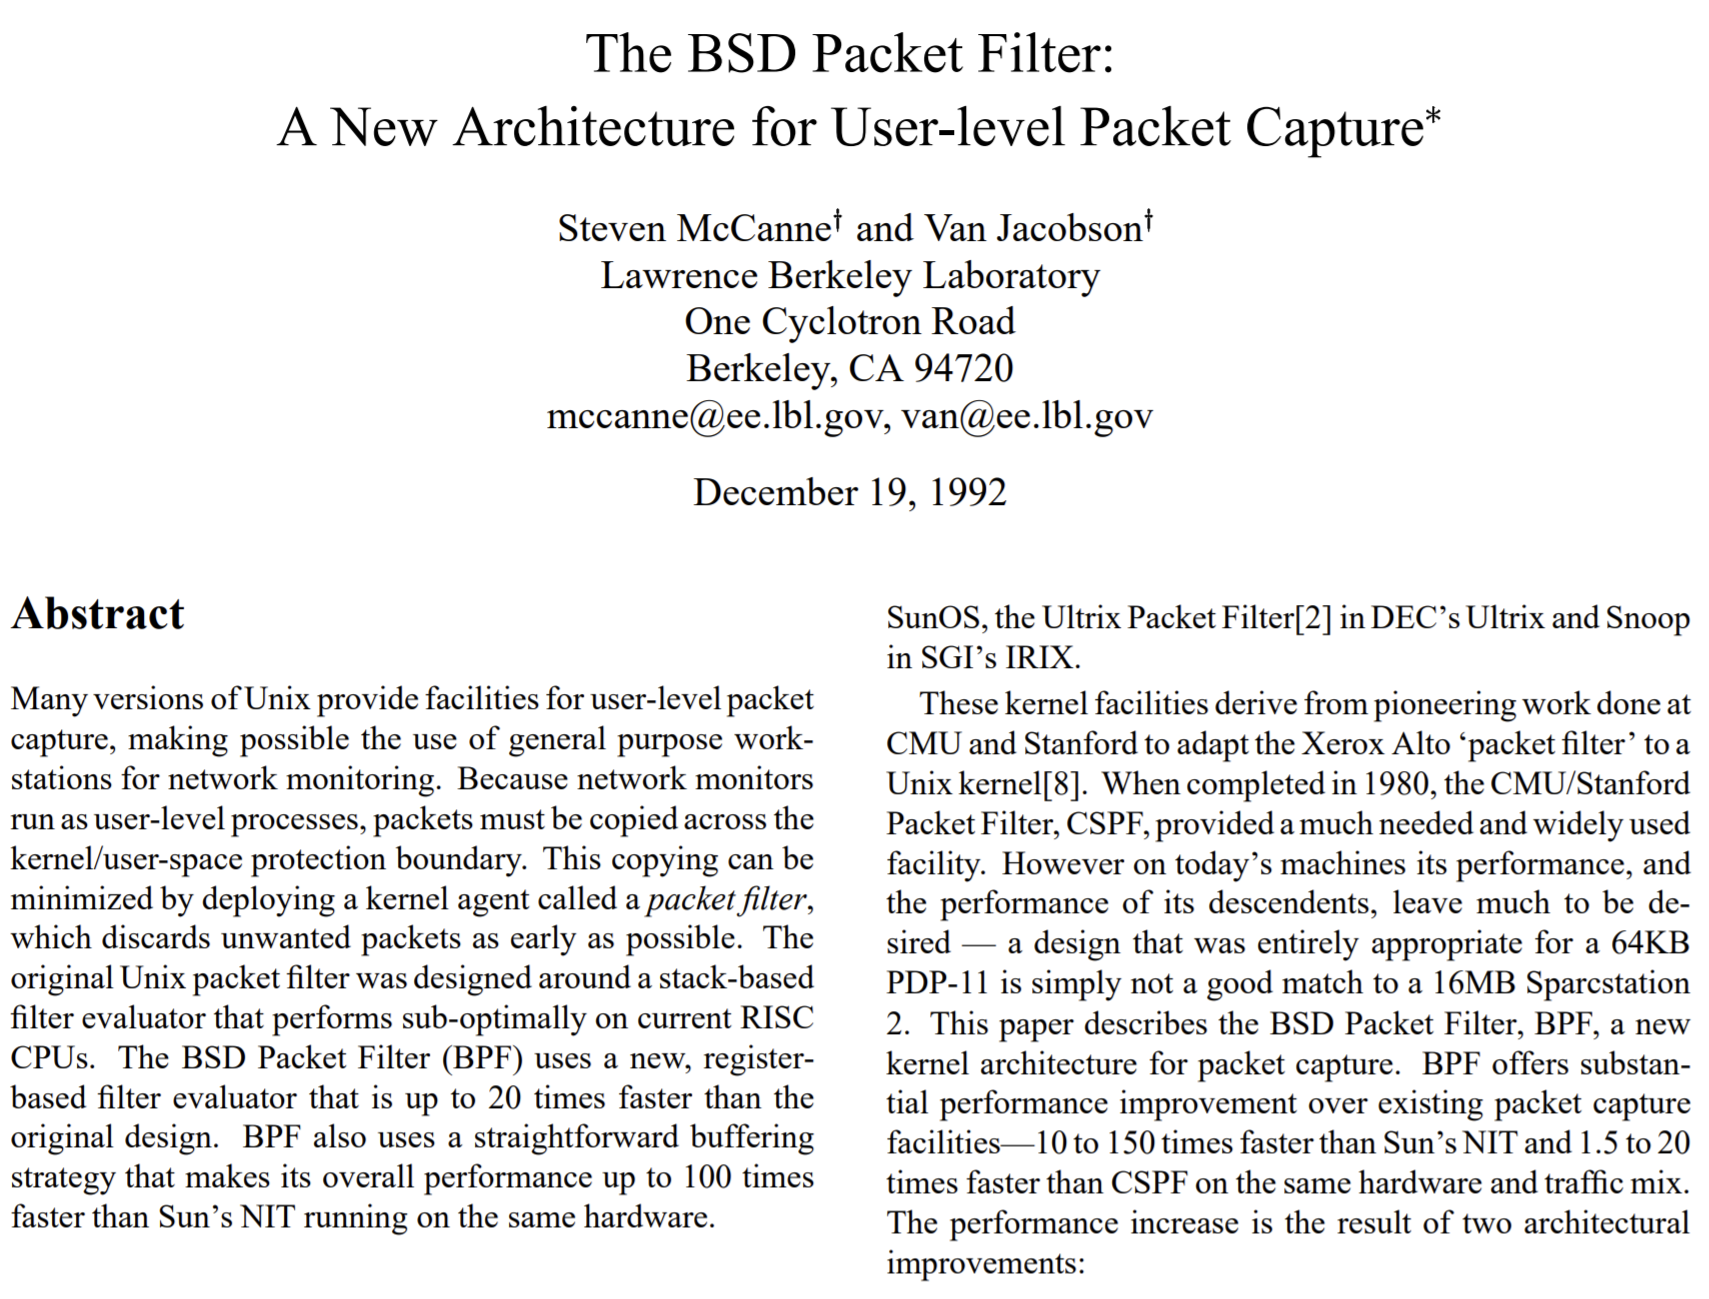
\includegraphics[height=6cm]{bpf_paper.png}
\end{center}
\end{frame}

% You can reveal the parts of a slide one at a time
% with the \pause command:
\begin{frame}{BPF}{A simple virtual machine residing in the kernel}
\begin{center}
    \includegraphics[height=7cm]{bpf_isa.png}
\end{center}
\end{frame}

\begin{frame}{How Does a BPF program work?}{Let's take a digression first}
How do userspace programs work ?

\begin{exampleblock}{Compiled}
Write Code $\rightarrow$ Compiler + Linker $\rightarrow$ Run the Binary
\end{exampleblock}

\begin{exampleblock}{Interpreted}
Write Code $\rightarrow$ Interpreter $\rightarrow$ JIT instruction $\rightarrow$ execute JIT-ed instructions
\end{exampleblock}
\hrulefill

\LARGE But wait the BPF VM is in the \alert{kernel}!


\end{frame}

\begin{frame}{BPF}{How does a BPF program run ?}
BPF a.k.a Classical BPF (cBPF) programs are STATELESS.\newline
Hook points are \alert{only} in the \alert{Network Stack}.
\begin{columns}
\begin{column}{0.6\textwidth}
\begin{itemize}
    \item Write a simple program (Filter) using the ISA.
    \item Filter expressions return True/False.
    \item \alert{Load} the ByteCode program in the kernel.
    \item \alert{Attach} the loaded program to a hook. (e.g on every received packet)
    \item Programs are \alert{event driven} and are \alert{run to completion} when the event occurs.
\end{itemize}
\end{column}
\begin{column}{0.4\textwidth}
    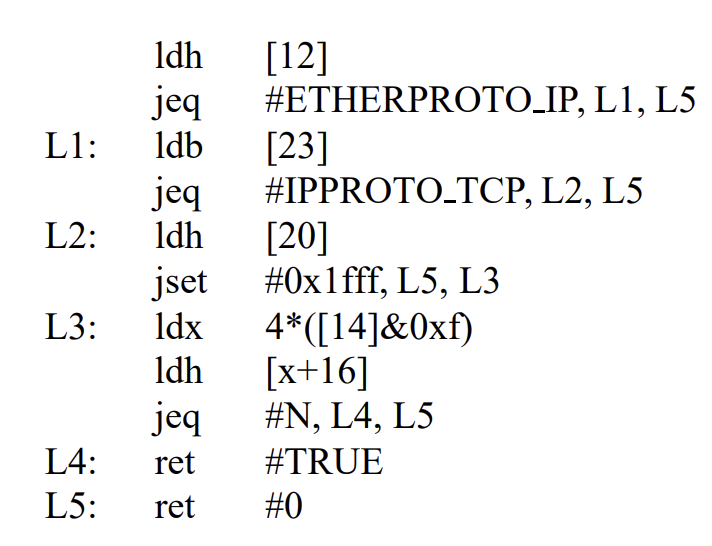
\includegraphics[height=3.5cm]{filter.png}
\end{column}

\end{columns}

\begin{exampleblock}

Load Byte Code $\rightarrow$ Interpreter $\rightarrow$ Attach to Hook $\rightarrow$ Run BPF $\rightarrow$ Action
\end{exampleblock}
\end{frame}

\begin{frame}{Ideas Similar to BPF}{Do not map 1:1 exactly -- similar theme}
\Large
\begin{itemize}
    \item Embeded \alert{lua} VM in nginx to modify behaviour without recompiling nginx or writing C.
    \item Embeded \alert{lua} VM in neovim to write plugins and extend functionality.
    \item Vimscript for VIM to extend functionality.
    \item Writing WebAssembly filters for \alert{envoy} proxy.
    \item WebAssembly for browsers.
\end{itemize}
    
\end{frame}


\section{Foundations}
\subsection{eBPF Architecture}
\begin{frame}{eBPF Mascot}{The cute Bee!}
    \centering
    
\includegraphics[width=12cm]{logo.png}
\end{frame}

\begin{frame}{extended BPF}{BPF VM in the Linux Kernel got improved vastly}
Alexei Starovoitov sent a patch improving the existing BPF infrastructure in the kernel and as a result BPF $\rightarrow$ \alert{e}BPF.
\begin{figure}
    \centering
    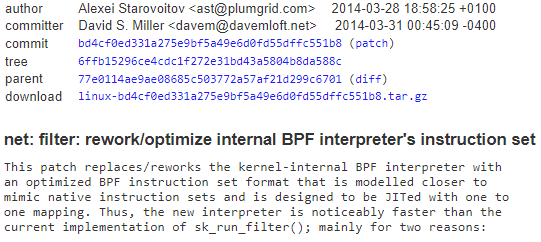
\includegraphics[height=5cm]{ebpf_linux.png}
\end{figure}
\end{frame}

\begin{frame}{extended BPF}{eBPF is not limited to the network stack\footnote{Image courtesy http://ebpf.io}}
Recall \alert{cBPF} had hooks only in the network stack. \alert{eBPF} has hook points all throughout the kernel. 
\begin{figure}
    \centering
    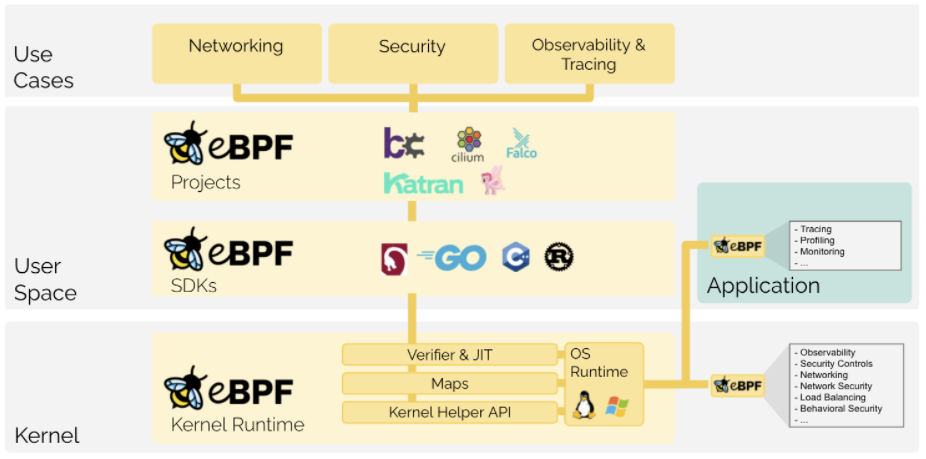
\includegraphics[height=5cm]{ebpf.png}
\end{figure}
\end{frame}

\begin{frame}{eBPF Capabilities}{Having a secure VM in the kernel has endless possibilities \footnote{Image courtesy http://ebpf.io}}
\begin{columns}
\begin{column}{0.5\textwidth}
\begin{figure}
    \centering
    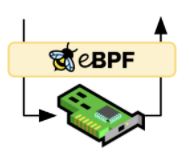
\includegraphics[height=2.5cm]{e_networking.png}\newline Networking
\end{figure}
\begin{figure}
    \centering
    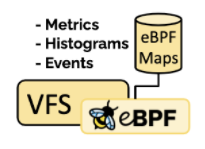
\includegraphics[height=2.5cm]{e_olly.png}\newline Observability
\end{figure}

\end{column}

\begin{column}{0.5\textwidth}
\begin{figure}
    \centering
    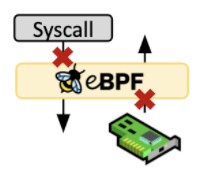
\includegraphics[height=2.5cm]{e_sec.png}\newline Security
\end{figure}
\begin{figure}
    \centering
    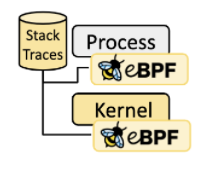
\includegraphics[height=2.5cm]{e_tracing.png}\newline Tracing
\end{figure}

\end{column}
\end{columns}
\end{frame}

\begin{frame}{eBPF Verifier \& JIT}{Loading and Attaching a eBPF program\footnote{Image courtesy http://ebpf.io}}
The \alert{bpf()} syscall is a multi-tool which lets us load \& attach an eBPF program.
\begin{figure}
    \centering
    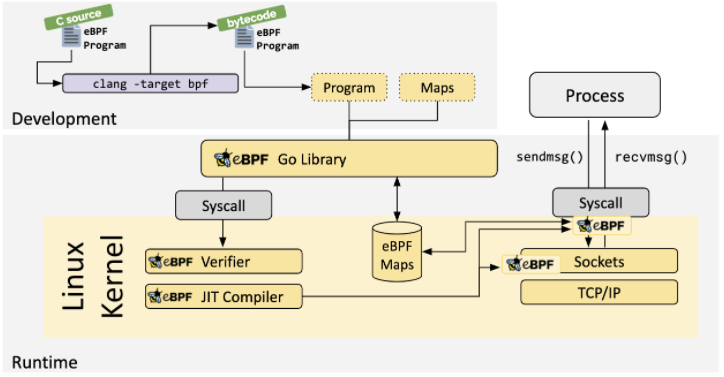
\includegraphics[height=5cm]{e_verifier_jit.png}
\end{figure}
\end{frame}

\subsection{eBPF Prog Types}
\begin{frame}{eBPF Program Types}{Different kinds of eBPF programs}
A non exhaustive list of \alert{BPF\_PROG\_*}:
\vspace{0.5cm}
\begin{itemize}
    \item BPF\_PROG\_TYPE\_SOCKET\_FILTER: a packet filter
    \item BPF\_PROG\_TYPE\_XDP: a packet filter run from device driver rx path
    \item BPF\_PROG\_TYPE\_KPROBE: if a kprobe should fire or not
    \item BPF\_PROG\_TYPE\_TRACEPOINT: if a tracepoint should fire or not
    \item BPF\_PROG\_TYPE\_SOCK\_OPS: set socket options
    \item BPF\_PROG\_....
    
\end{itemize}
\end{frame}

\subsection{eBPF Maps}
\begin{frame}{eBPF MAPs}{Saving State in eBPF Programs}
Recall \alert{cBPF} was entirely stateless. \alert{eBPF} is stateless but has the capability to access storage which are called eBPF MAPs. eBPF MAP is a generic data structure that allows data to be passed back and forth withing the kernel or between the user space and the kernel.

eBPF MAPS are created by the same \alert{bpf()} syscall.

\vspace{0.5cm}
A few interesting \alert{BPF\_MAP\_TYPE\_*}:
\begin{itemize}
    \item BPF\_MAP\_TYPE\_HASH: an actual hash table
    \item BPF\_MAP\_TYPE\_ARRAY: an array
    \item BPF\_MAP\_TYPE\_PROG\_ARRAY: an array of fd's corresponding to eBPF programs.
    \item BPF\_MAP\_TYPE\_...
\end{itemize}
\end{frame}

\begin{frame}{Thank You!}
\centering

\includegraphics[height=5cm]{questions.png}
\end{frame}

\end{document}
